\section{Measurements}
\label{sec:measurements}

\subsection{Preparations and calibration of the setup}
\label{sub:preparations_and_calibration_of_the_setup}
\subsubsection{Controlling the setup with the oscilloscope}
\label{ssub:Controlling the setup with the oscilloscope}
The parameters set for the first configuration are shown in table~\ref{tab:config}. 
First we measured the signal from the detector and photomultiplier. We noticed
that the peaks of shape a) and b) were at irregular points in time (see figure \ref{fig:osci}). 
We changed the input from the left to the right detector but did not observe a appreciable differences.
Rotating the sample did not change the result significantly, either. 
\\
\\
 \begin{minipage}{\textwidth}
  \begin{minipage}[b]{0.49\textwidth}
    \centering
    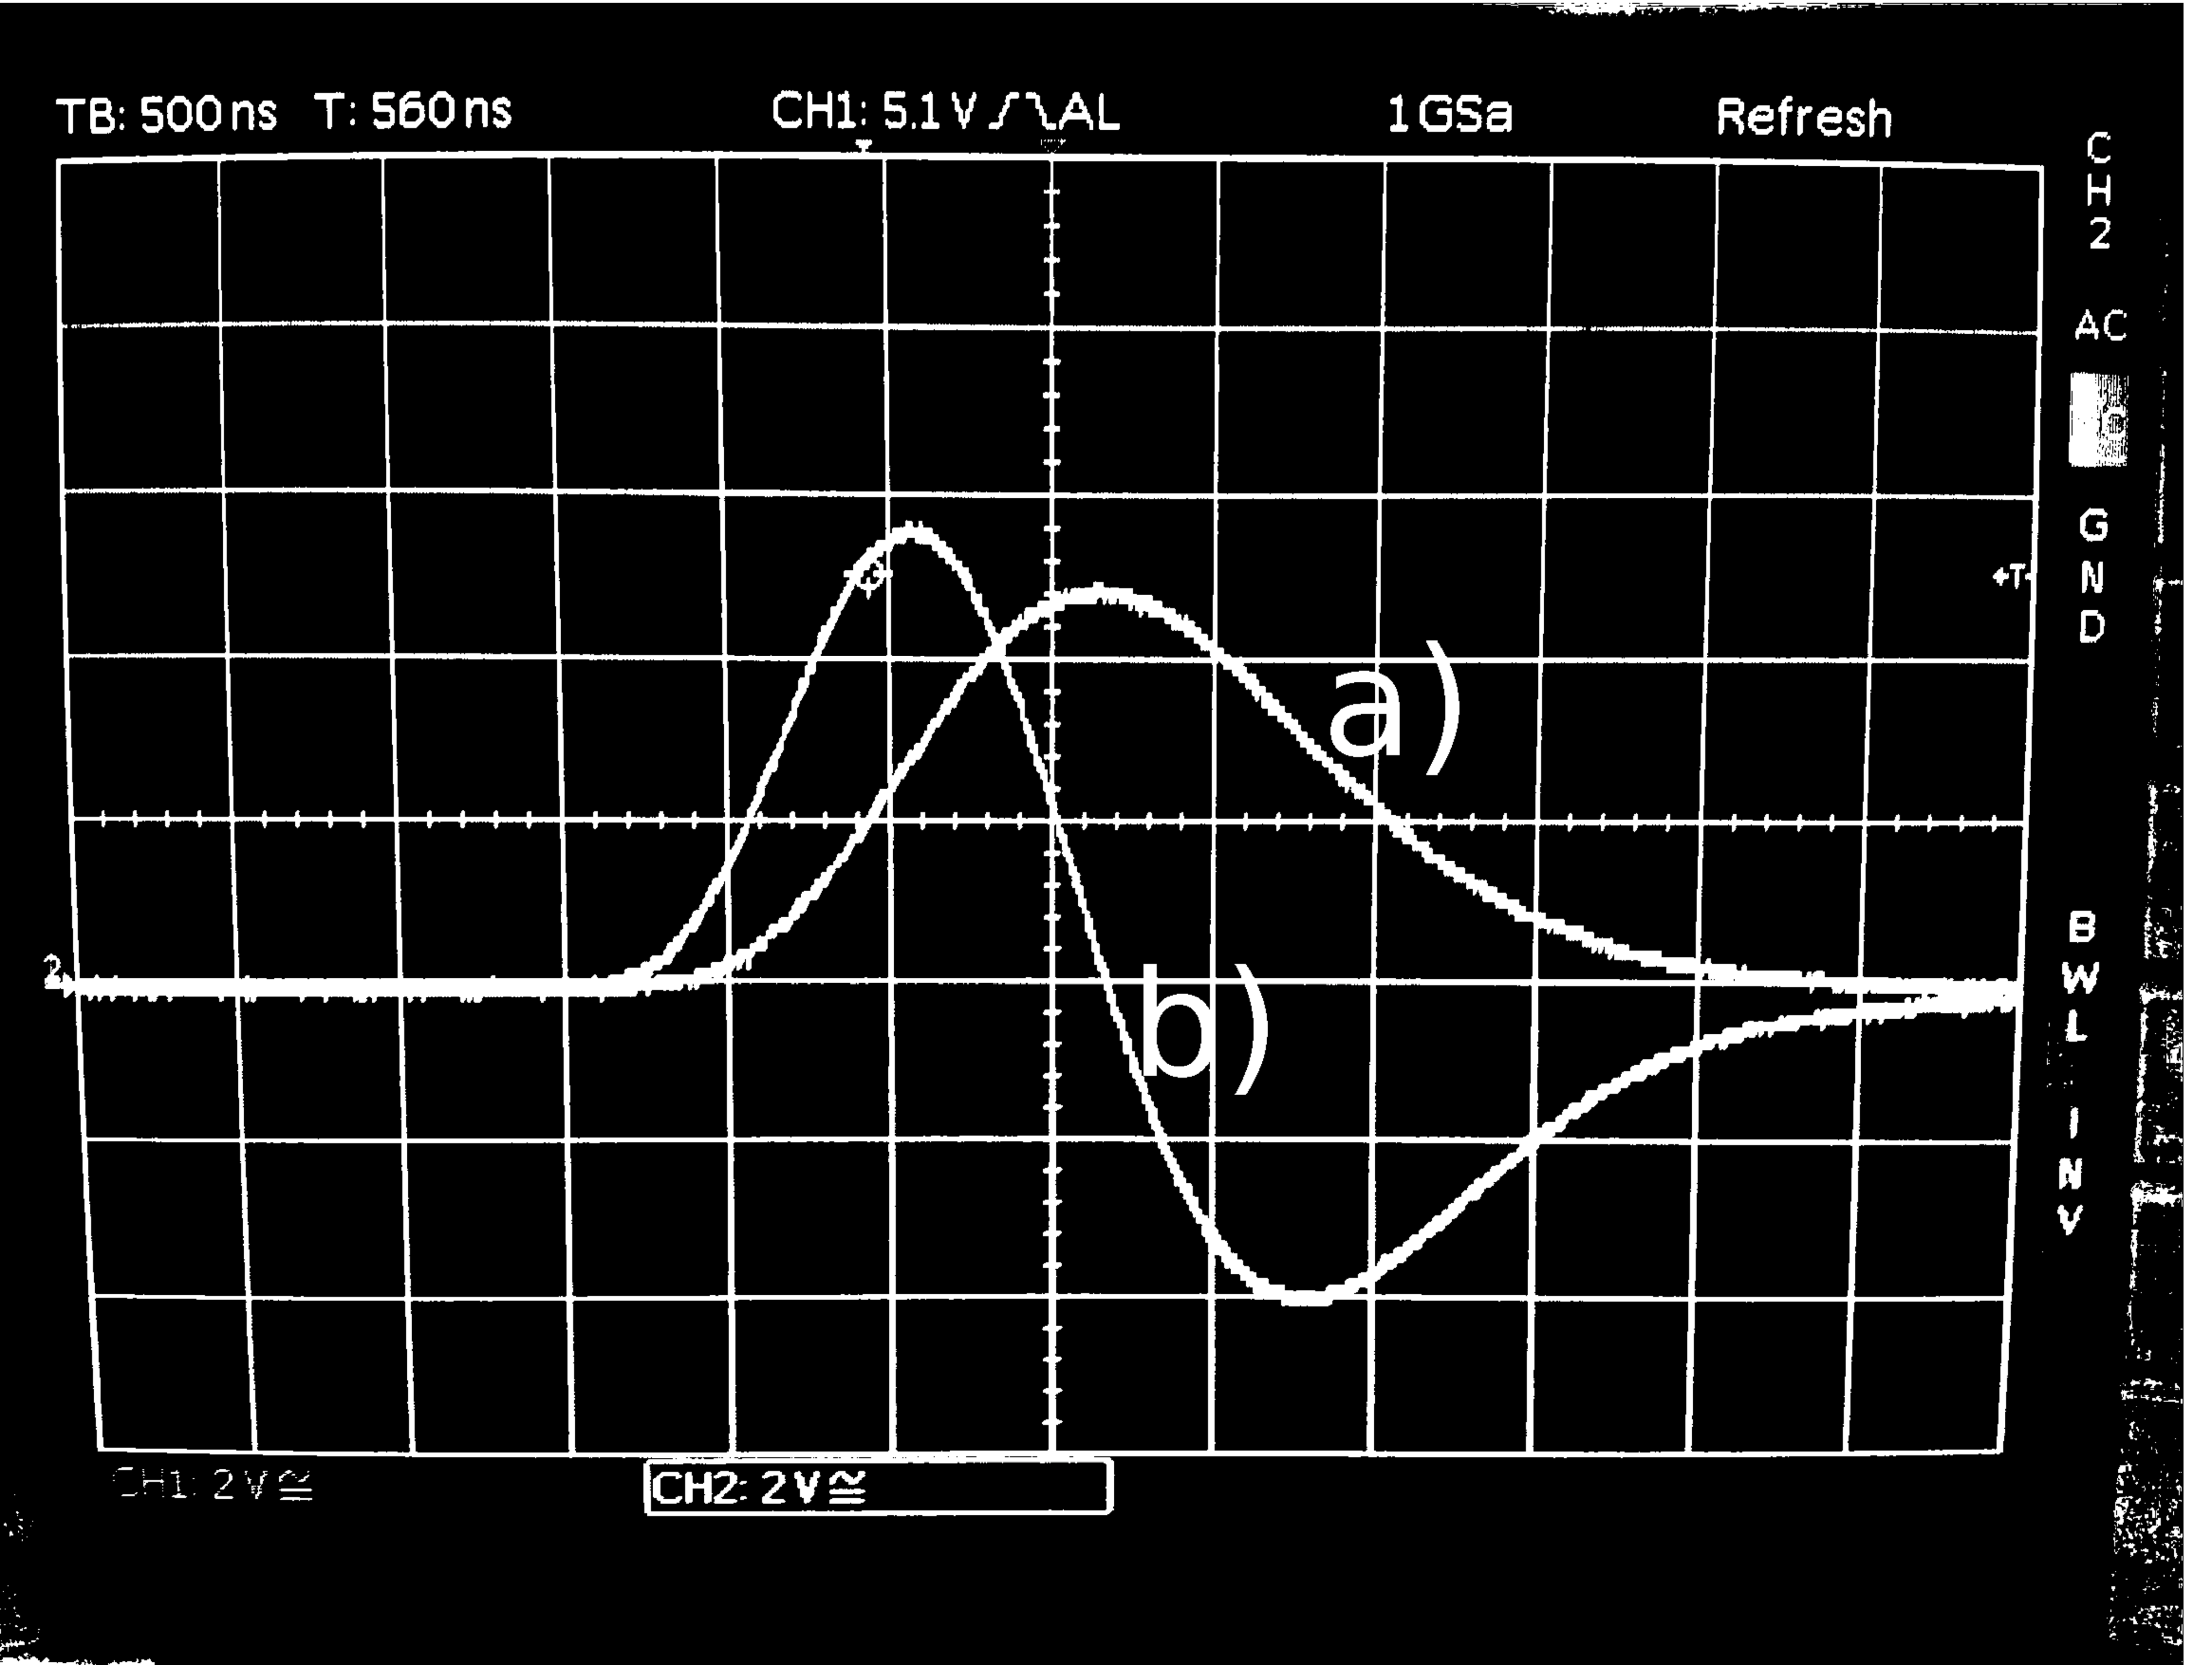
\includegraphics[width=0.8\linewidth]{figures/uni_bipolar2}
    \captionof{figure}{Oscillscope: a) refers to the unipolar channel and b) to 
        the bipolar channel.}
    \label{fig:osci}
  \end{minipage}
  \hfill
  \begin{minipage}[b]{0.49\textwidth}
    \centering
 \begin{tabular}{|l|l|}
     \hline
    course grain & 100\\
    gain    &   10.0 \\
    sharpening time &   0.5 \\
    sample & position 1\\
    PM & Right Side\\
    output & unipolar MCA\\
           & bipolar delay\\
     BLR & AFJ \\
     +/- & Pos \\
     delay & out\\
     \hline
\end{tabular}
\label{tab:config}
  \captionof{table}{Configuration of MA, MCA in measurement 2.1.1.}
    \end{minipage}
\end{minipage}

\subsubsection{Measuring the full energy spectrum}
\label{ssub:Measuring the full energy spectrum}
In the next step, we removed the oscilloscope and connected the multichannel analyzer (MA)
in order to measure the energy spectrum. In order to be able to decide which detector and position would
be suitable, we increased gain and coarse gain of the MA to 8.6 and 200, respectively.
This way, the observed spectrum was distributed over the entire range of bins. 
The setup is listed in table~\ref{tab:config2}. With the four possible combinations
of position and detector, we obtained four different histograms, shown in figure~\ref{fig:measure2.1}.
For the further measurements, we chose detector +++??? for the lower and much less 
pronounced peak, since it show a higher sensibility in that region. The 
chosen position for the sample is thus +++???.
\begin{table}[htp]
    \begin{tabular}{|l|l|l||l|l|l|}
        \hline
        2.1a) & Positions:  & Pos1         & 2.1b) & Positions:  & Pos1\\
              & PM          & right        &       & PM          & left \\
              & Time        & $360\pm1$sec &       & Time        & $380\pm1$sec \\
        \hline 
        2.1c) & Positions:  & Pos2         & 2.1d) & Positions:  & Pos2         \\
              & PM          & right        &       & PM          & left \\
              & Time        & $402\pm1$sec &       & Time        & $368\pm1$sec \\
        \hline 
        2.1e) & Positions:  & Pos2         \\
              & PM          & left \\
              & Time        & $360\pm1$sec \\
    \cline{1-3}
    \end{tabular}
  \caption{Configuration in measurement 2.1 of position, PM and integration time.}
    \label{tab:config2}
\end{table}

\begin{figure}
    \begin{subfigure}[b]{\picwidth}
        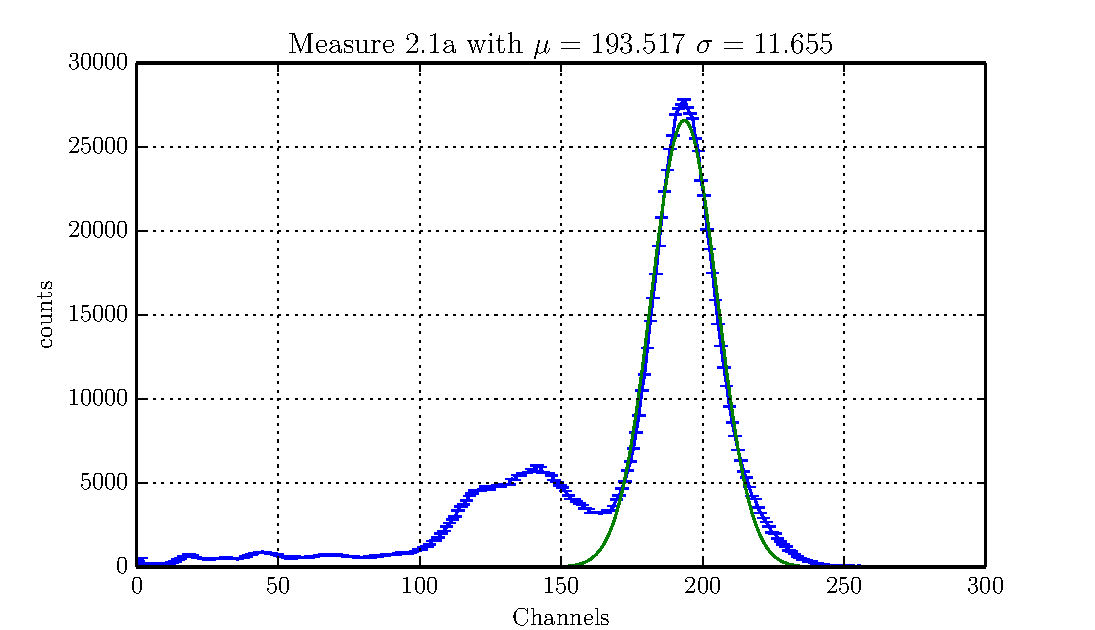
\includegraphics[width=\textwidth]{analysis/figures/plot2_1a}
        \caption{}
    \end{subfigure}\qquad
    \begin{subfigure}[b]{\picwidth}
        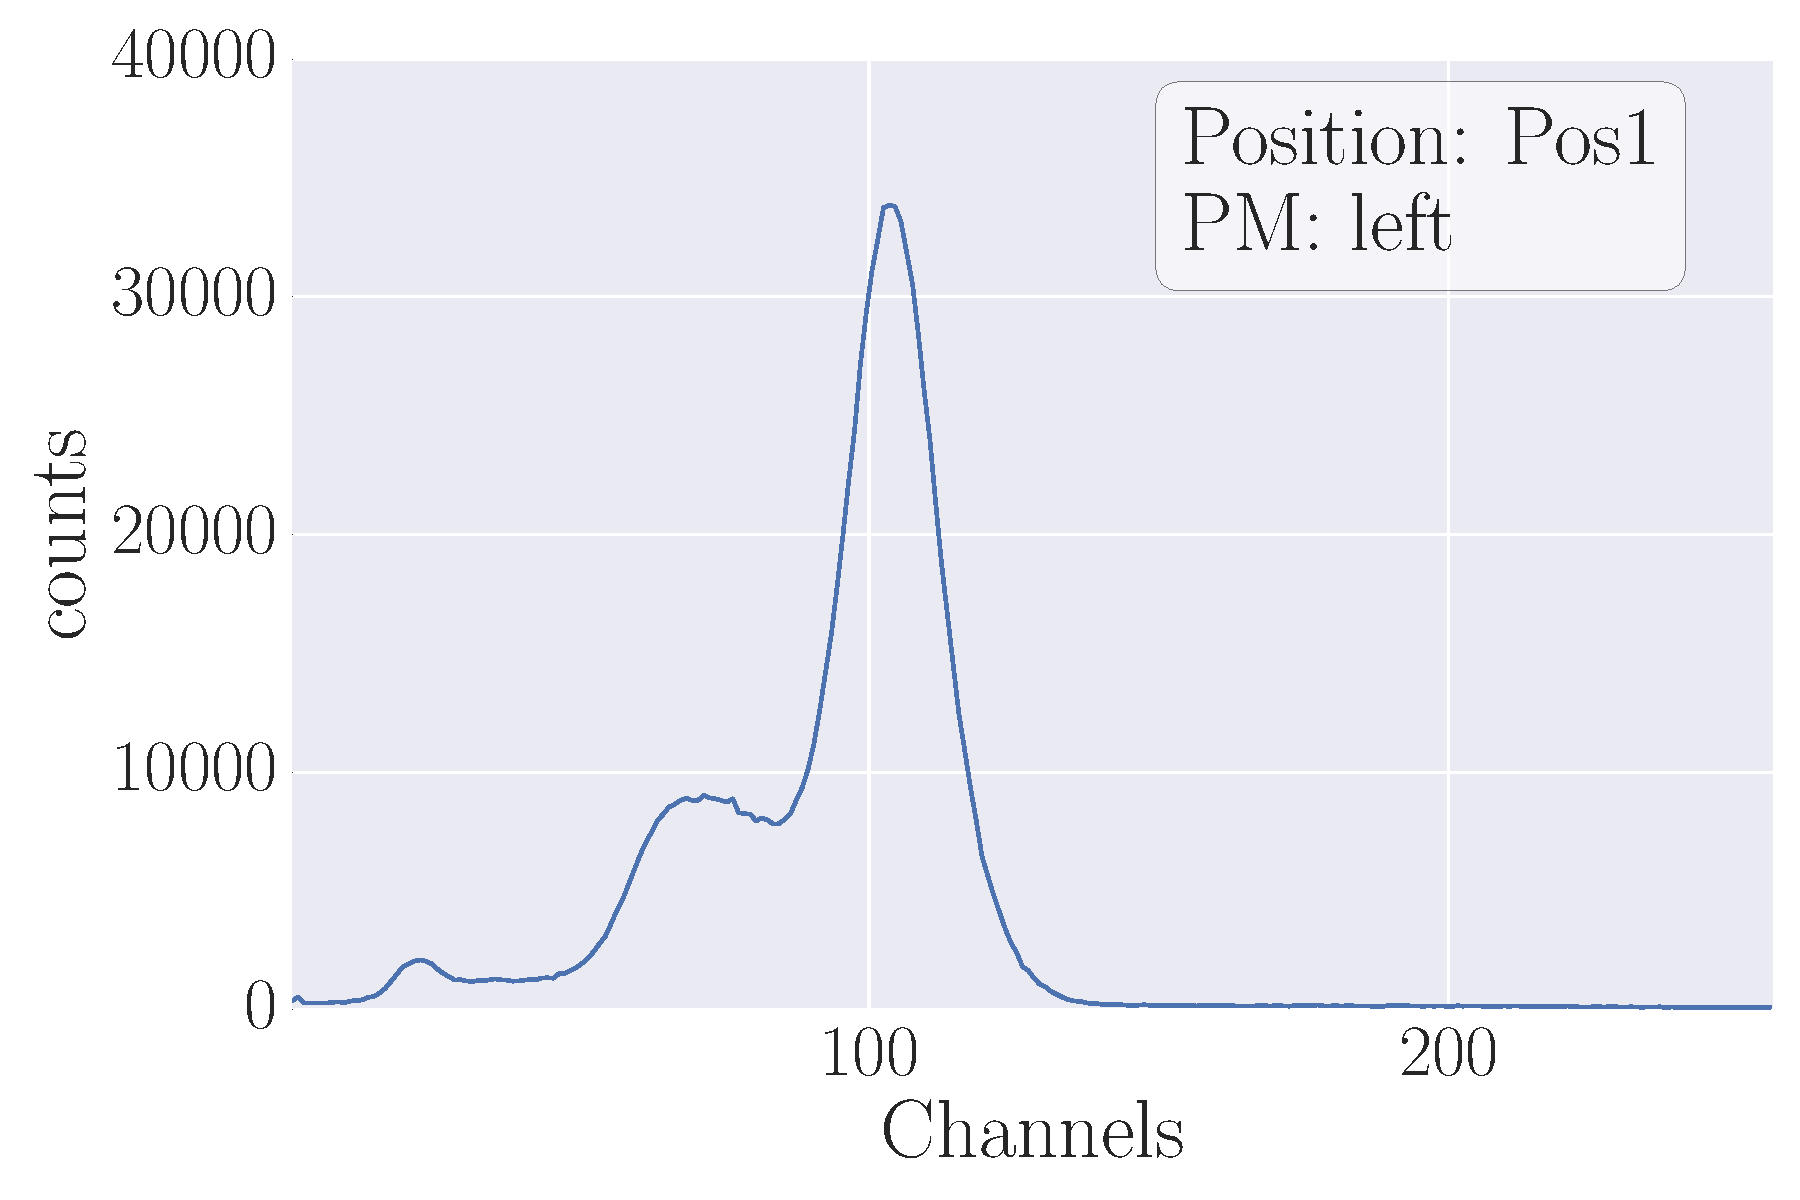
\includegraphics[width=\textwidth]{analysis/figures/plot2_1b}
        \caption{}
    \end{subfigure}
    \begin{subfigure}[b]{\picwidth}
        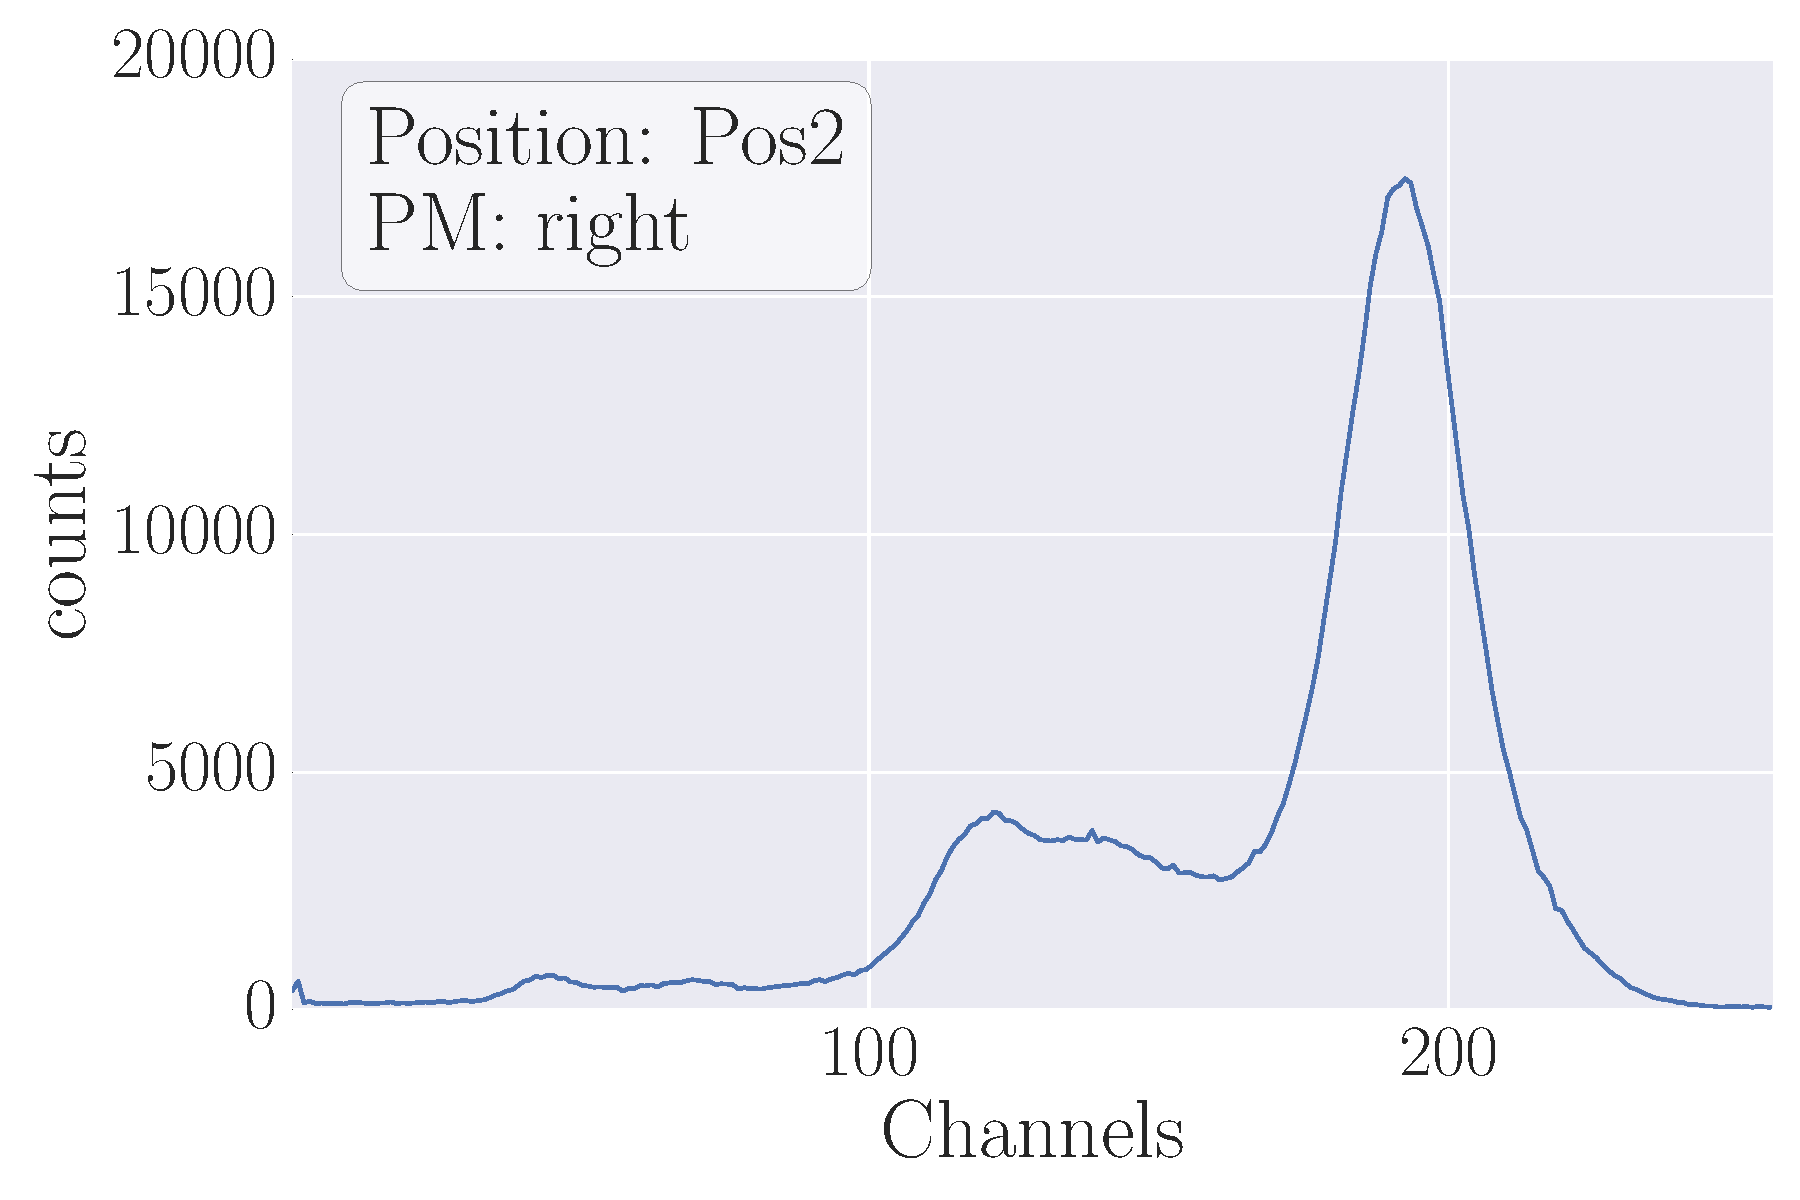
\includegraphics[width=\textwidth]{analysis/figures/plot2_1c}
        \caption{}
    \end{subfigure}
    \begin{subfigure}[b]{\picwidth}
        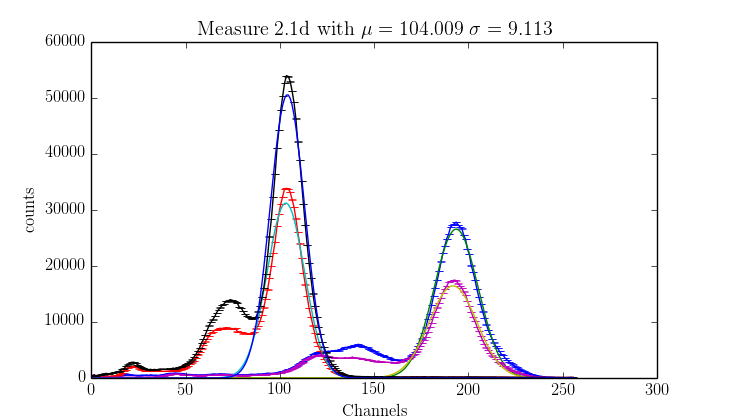
\includegraphics[width=\textwidth]{analysis/figures/plot2_1d}
        \caption{}
    \end{subfigure}
    \begin{subfigure}[b]{\picwidth}
        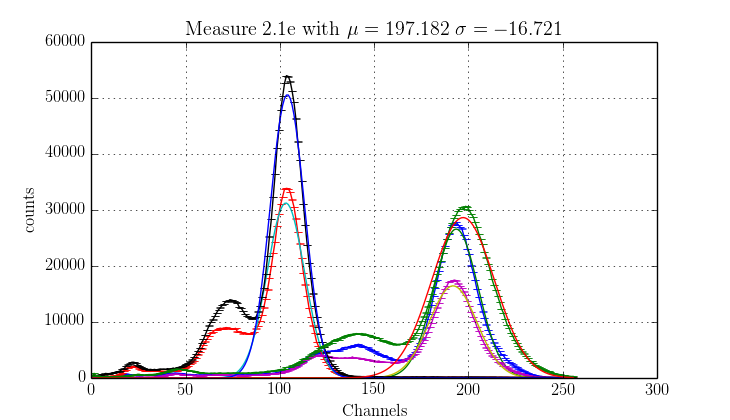
\includegraphics[width=\textwidth]{analysis/figures/plot2_1e}
        \caption{}
    \end{subfigure}
    \caption{
        Histograms of events recorded with the MCA, thus corresponding to the energy 
        spectrum of the probe. Each histogram corresponds to a combination of position 
        of the probe and used detector, as classified in table \ref{tab:config2}
        }
    \label{fig:measure2.1}
\end{figure}
\clearpage
\subsection{Measuring $\Delta t$ of coincidences}

\subsubsection{Calibration of TAC-MCA Signal}
\label{subs:calib_TAC}
In order to relate the channels to the delay, we used the following
measurement for calibration. We used a least square fit for the parameters
of the linear relation:
\begin{align}
    \label{eq:coeff}
    y &= ax + b \\
    a &= \left[ 1.315 \pm 0.005 \right] \mathrm{ns} / \mathrm{Channel}\\
    b &= \left[ -22.6 \pm 0.5 \right]\mathrm{ns} 
\end{align}
where the $x$-values are given by the number of the corresponding channel. 
The resulting covariance matrix of the fit is the following:
\begin{align}
    \label{eq:cov}
    \mathrm{cov}(a, b) &=& 
    \begin{pmatrix}
        2.318 \cdot 10^{-5}\mathrm{ns}^2 &-2.089\cdot 10^{-3}\mathrm{ns}^2\\
        -2.089\cdot 10^{-3}\mathrm{ns}^2&2.328\cdot 10^{-1}\mathrm{ns}^2\\
    \end{pmatrix}
\end{align}
where the units correspond to those of $a$ and $b$ 
(e.~g. $\mathrm{cov}(a,a) = 2.318\mathrm{e}-05 \mathrm{ns^2} / \mathrm{Channel}^2$).
The $\chi^2$-test results in:
\begin{align}
    \label{eq:}
   \chi^2 = 0.972
\end{align}

\label{sub:calibration_of_tac_mca_signal}
\begin{figure}[htpb]
    \centering
    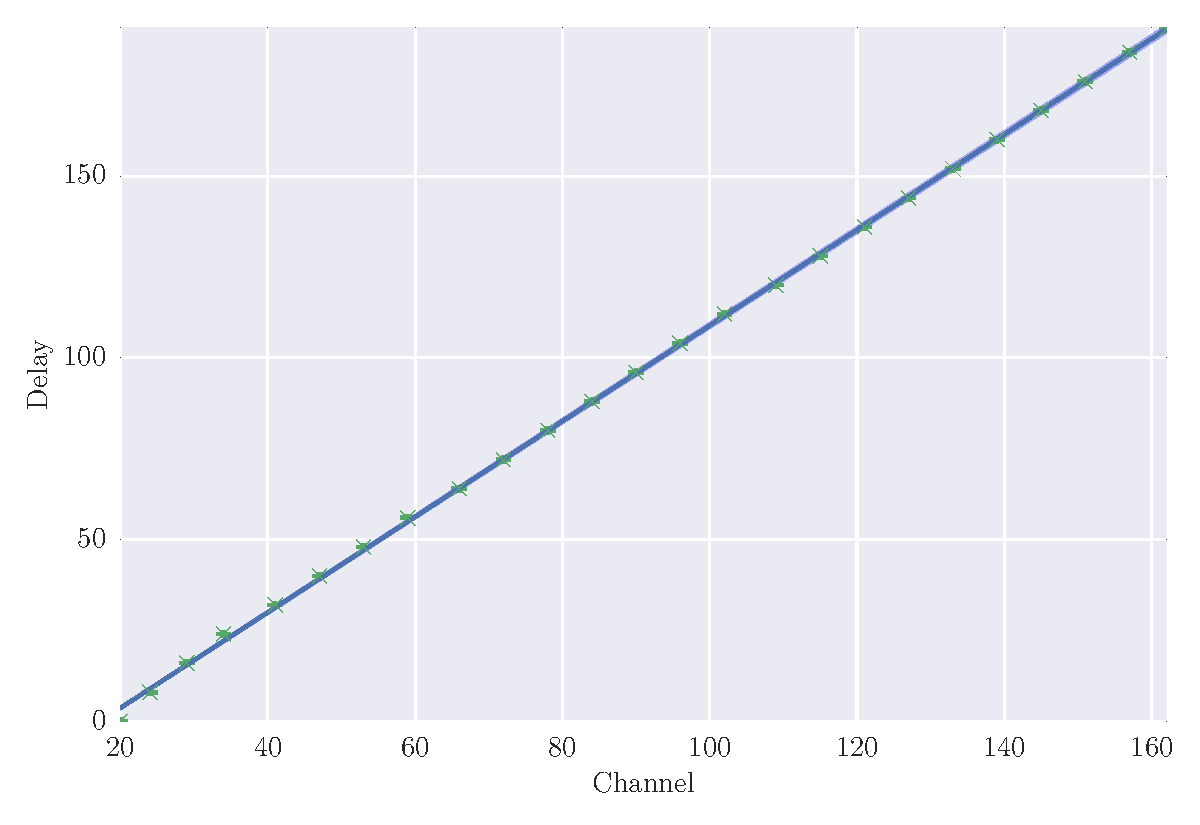
\includegraphics[width=1.0\linewidth]{analysis/figures/plot7}
    \caption{Calibration of the TAC-MCA Signal. The errorbars are too small
        to see clearly, since the $\chi^2$ test ist also nearly 1.}
    \label{fig:plot7}
\end{figure}



\label{sub:measuring_delayed_coincidences}
\subsubsection{Setting the energy window}
\label{ssub:Setting the energy window}
Setting the windows for the chosen combination of smaple position and detectors did 
not work out right away. In a first attempt, we selected the wrong lower peak (see appendix 
    \ref{sec:appendix} for the corresponding settings). 
The second run turned out to be more successful, however. The corresponding configuration is 
shown in the tables below. For the the time delay we chose
$\Delta t = 140$ns.\\\\ 
 \begin{minipage}{\textwidth}
  \begin{minipage}[b]{0.49\textwidth}
   \begin{tabular}{|l|l|}
        \hline
       14.4 keV signal & right detector \\
       122 keV signal & left detector \\
       coarse gain & 200 \\
       gain & 8.6 \\
       Shaping time & $0.5\mu$s \\
        \hline
   \end{tabular}

  \captionof{table}{Configuration of MA1}
  \end{minipage}
  \hfill
  \begin{minipage}[b]{0.49\textwidth}
    \centering
   \begin{tabular}{|l|l|}
        \hline
       Lower Level & $4.75\pm0.05$ \\
       Upper Level & $3.72\pm0.05$ \\
       Delay & 1.0 (minimum possible) \\
        walk ADJ & $0.1 - 1.1\mu$s (NOR)  \\
       Pos Out & Linear Gate ``enable''\\
        \hline
   \end{tabular}
  \captionof{table}{Configuration of SCA1}
\end{minipage}
\end{minipage}
\begin{minipage}{\textwidth}
  \begin{minipage}[b]{0.49\textwidth}
   \begin{tabular}{|l|l|}
        \hline
       coarse gain & 500 \\
       gain & 8.6 \\
       Shaping time & $0.5\mu$s \\
       input & right detector \\ 
        delay & out \\
        \hline
   \end{tabular}

  \captionof{table}{Configuration of MA2}
  \end{minipage}
  \hfill
  \begin{minipage}[b]{0.49\textwidth}
    \centering
   \begin{tabular}{|l|l|}
        \hline
       Lower Level & $2.02\pm0.05$ \\
       Upper Level & $3.04\pm0.05$ \\
       Delay & 1.0 (minimum possible) \\
        walk ADJ & $0.1 - 1.1\mu$s (NOR)  \\
       Pos Out & Linear Gate ``enable''\\
        \hline
   \end{tabular}
  \captionof{table}{Configuration of SCA2}
\end{minipage}
\end{minipage}
\clearpage
\subsubsection{Delayed coincidences}
The measurement ran about 14 hours over night. See Figure~\ref{fig:4_1} for the visualization.
\label{ssub:Conduction of the experiment over night}

\begin{figure}[htpb]
    \centering
    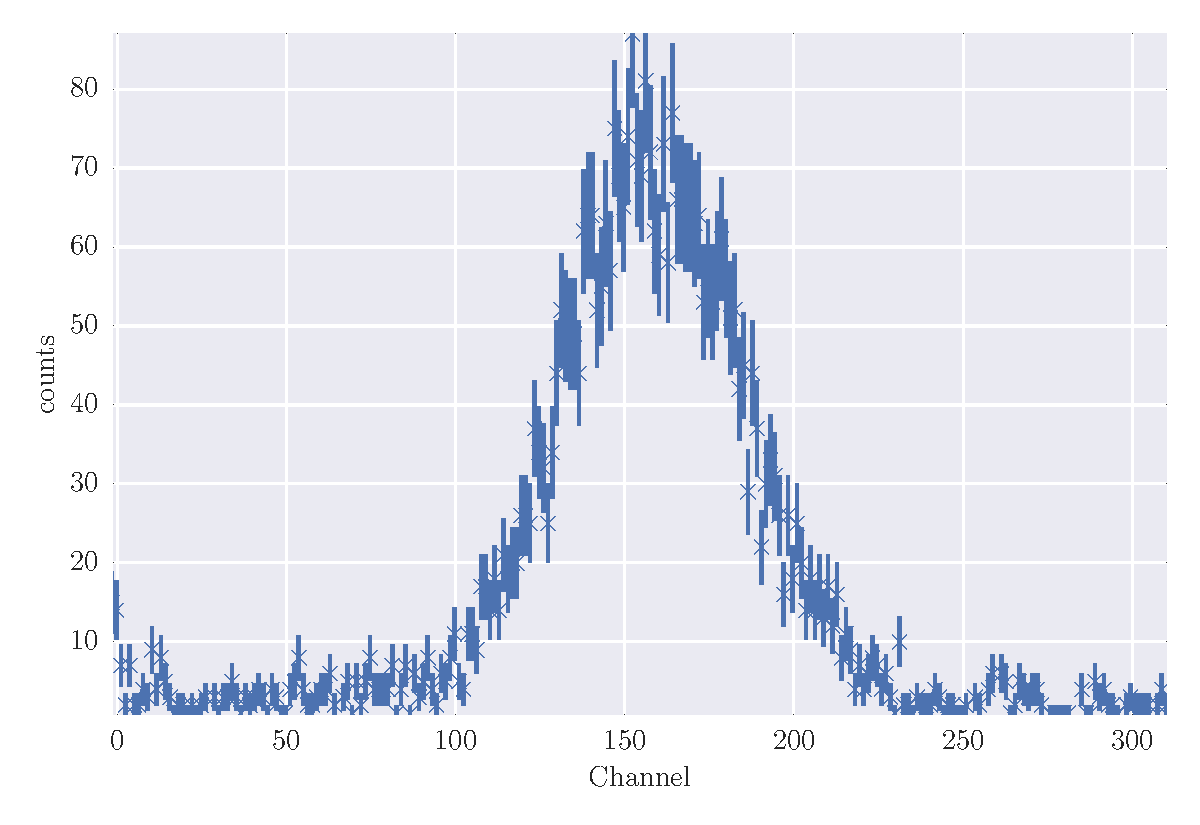
\includegraphics[width=1.0\linewidth]{analysis/figures/plot4_1}
    \caption{Measurement 4.1: You will notice that the shape
        of the peak looks gaussian, which is rather unexpected. However
        further analysis show, that the peak is not symmetric and hence the left 
        side will be fitted against a exponential curve, while the origin of the
        right side is the background, which will be analyzed in the next section.
        The errors which are visualized here are approximated by $S_{N_i} = \sqrt{N_i}$.}
    \label{fig:4_1}
\end{figure}
\clearpage
\subsubsection{Random coicidences}
\label{ssub:Random coicidences}
For measuring the background we used the same configuration as before, except of the TAC-input:
\begin{itemize}
    \item TAC Start: SCA2, triggered by the 14.4 keV Peak, delayed with $\Delta t = 48$ns
    \item TAC Stop: SCA1, triggered by 122 keV (no delay)
\end{itemize}
A first approach with $\Delta t = 16$ns failed, since we observed a clear peak in low channels in contrary
to an expected equally distributed signal. After changing to $\Delta t=48$ns we observe a clear
background noise signal, which you can see in Figure~\ref{fig:5_1}.
\begin{figure}[htpb]
    \centering
    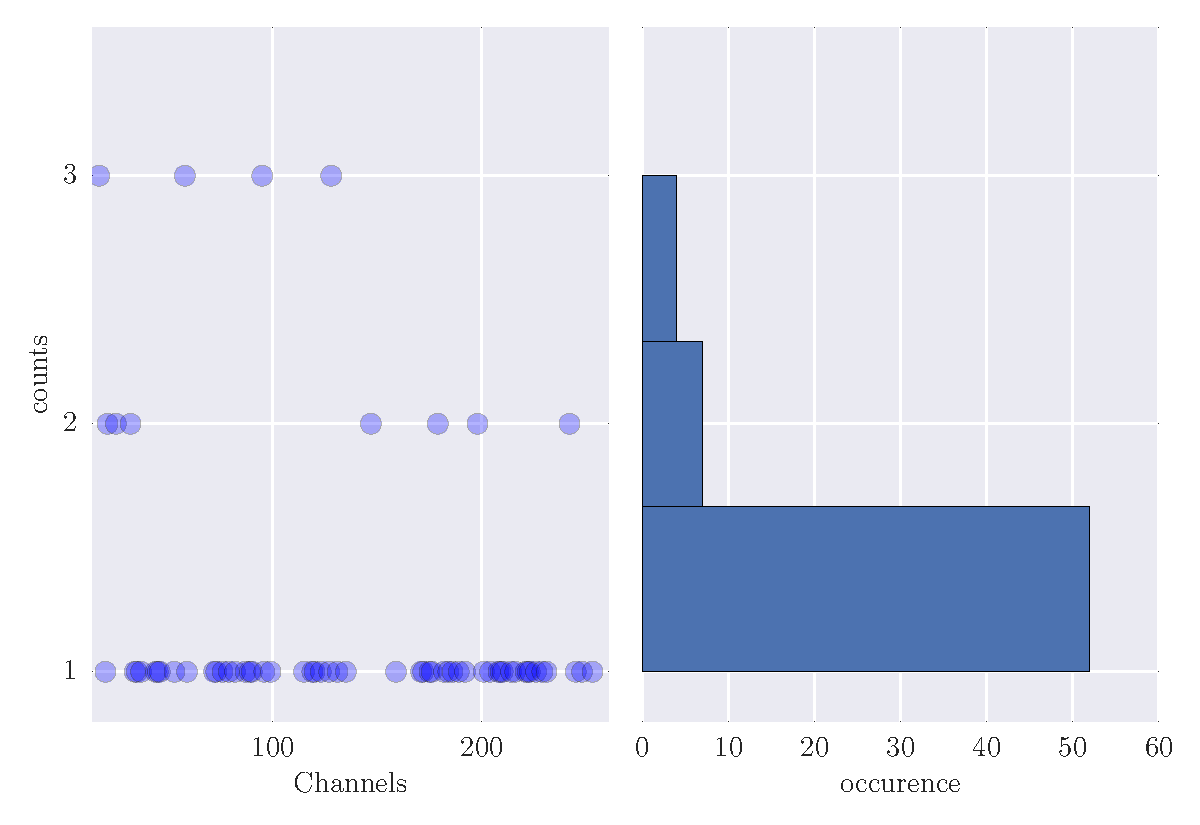
\includegraphics[width=1.0\linewidth]{analysis/figures/plot5_1_hist}
    \caption{Measurement 5.1: Random coincidences and their histogram.}
    \label{fig:5_1}
\end{figure}
\clearpage

